\documentclass[ignorenonframetext,]{beamer}
\setbeamertemplate{caption}[numbered]
\setbeamertemplate{caption label separator}{:}
\setbeamercolor{caption name}{fg=normal text.fg}
\usepackage{amssymb,amsmath}
\usepackage{ifxetex,ifluatex}
\usepackage{fixltx2e} % provides \textsubscript
\usepackage{lmodern}
\ifxetex
  \usepackage{fontspec,xltxtra,xunicode}
  \defaultfontfeatures{Mapping=tex-text,Scale=MatchLowercase}
  \newcommand{\euro}{€}
\else
  \ifluatex
    \usepackage{fontspec}
    \defaultfontfeatures{Mapping=tex-text,Scale=MatchLowercase}
    \newcommand{\euro}{€}
  \else
    \usepackage[T1]{fontenc}
    \usepackage[utf8]{inputenc}
      \fi
\fi
% use upquote if available, for straight quotes in verbatim environments
\IfFileExists{upquote.sty}{\usepackage{upquote}}{}
% use microtype if available
\IfFileExists{microtype.sty}{\usepackage{microtype}}{}
\usepackage{longtable,booktabs}
\usepackage{caption}
% These lines are needed to make table captions work with longtable:
\makeatletter
\def\fnum@table{\tablename~\thetable}
\makeatother
\usepackage{graphicx}
\makeatletter
\def\maxwidth{\ifdim\Gin@nat@width>\linewidth\linewidth\else\Gin@nat@width\fi}
\def\maxheight{\ifdim\Gin@nat@height>\textheight0.8\textheight\else\Gin@nat@height\fi}
\makeatother
% Scale images if necessary, so that they will not overflow the page
% margins by default, and it is still possible to overwrite the defaults
% using explicit options in \includegraphics[width, height, ...]{}
\setkeys{Gin}{width=\maxwidth,height=\maxheight,keepaspectratio}

% Comment these out if you don't want a slide with just the
% part/section/subsection/subsubsection title:
\AtBeginPart{
  \let\insertpartnumber\relax
  \let\partname\relax
  \frame{\partpage}
}
\AtBeginSection{
  \let\insertsectionnumber\relax
  \let\sectionname\relax
  \frame{\sectionpage}
}
\AtBeginSubsection{
  \let\insertsubsectionnumber\relax
  \let\subsectionname\relax
  \frame{\subsectionpage}
}

\setlength{\parindent}{0pt}
\setlength{\parskip}{6pt plus 2pt minus 1pt}
\setlength{\emergencystretch}{3em}  % prevent overfull lines
\setcounter{secnumdepth}{0}

\title{MRP y HMM}
\author{Andrea Fernández, Liliana Millán}
\date{27/05/2015}

\begin{document}
\frame{\titlepage}

\section{Aplicación 1: Modelo de reconocimiento de
vocales}\label{aplicacion-1-modelo-de-reconocimiento-de-vocales}

\begin{frame}{Problema}

Supongamos que somos alienígenas de Las Pléyades y que no tenemos ni
idea de cómo se `lee' un lenguaje de la tierra, no sabemos de los
idiomas pero como somos seres superiores sabemos de Hidden Markov
Models!

\begin{itemize}
\itemsep1pt\parskip0pt\parsep0pt
\item
  Objetivo:
\end{itemize}

Queremos establecer ciertas propiedades de este lenguaje que no
conocemos, veremos que al identificar estas propiedades, de manera
\emph{natural} identificaremos las vocales de las consonantes.

\end{frame}

\begin{frame}{Especificación del modelo}

\begin{itemize}
\itemsep1pt\parskip0pt\parsep0pt
\item
  Utilizamos HMM con el algoritmo Baum-Welch para estimar los
  parámetros:
\end{itemize}

\begin{enumerate}
\def\labelenumi{\arabic{enumi}.}
\itemsep1pt\parskip0pt\parsep0pt
\item
  las probabilidades inciales de los estados
\item
  las probabilidades de transición entre estados
\item
  las probabilidades de cada símbolo de pertenecer a uno de los estados
\end{enumerate}

\begin{itemize}
\itemsep1pt\parskip0pt\parsep0pt
\item
  Únicamente con la evidencia que tienen los datos (nuestras
  observaciones)
\end{itemize}

\end{frame}

\begin{frame}{Baum-Welch}

\begin{itemize}
\itemsep1pt\parskip0pt\parsep0pt
\item
  Este algoritmo es una variante del EM visto en clase. Iniciamos con un
  modelo sin `conocimiento'
\end{itemize}

$\pi$ = probabilidades de inciar en cada estado

A= matriz de transición de estados

B= matriz de emisiones

$\lambda=(A,B,\pi)$

\begin{itemize}
\itemsep1pt\parskip0pt\parsep0pt
\item
  En cada iteración los valores de $\pi$, A y B se van actualizando
  hasta convergencia
\item
  El algoritmo ocupa el forward procedure ---probabilidad de ver esta
  secuencia parcial y terminar en el estado i en el tiempo t--- y el
  backward procedure ---probabilidad de terminar en la esta secuencia
  parcial dado que empezamos en el estado i en el tiempo t---
\end{itemize}

\end{frame}

\begin{frame}{Datos}

\begin{itemize}
\itemsep1pt\parskip0pt\parsep0pt
\item
  Tomamos el corpus de noticias de periódicos españoles
\item
  309,918 noticias
\end{itemize}

\end{frame}

\begin{frame}{Limpieza de datos}

\begin{itemize}
\itemsep1pt\parskip0pt\parsep0pt
\item
  Eliminación de signos de puntuación
\item
  Eliminación de dígitos
\item
  Eliminación de tabuladores
\item
  Todas las letras a minúsculas
\item
  Cada palabra es separada en sus letras respetando los espacios
\end{itemize}

\end{frame}

\begin{frame}{Suposiciones iniciales del modelo}

\begin{itemize}
\item
  Nuestra base será suponer que existen 2 estados: \textbf{Consonante} y
  \textbf{Vocal}
\item
  No conocemos con qué probabilidad de inicio estamos en Constante o en
  Vocal
\item
  No conocemos las probabilidades de transición entre estados
\item
  No conocemos las probabilidades de que cada símbolo del lenguaje
  pertenezca a uno de los estados
\end{itemize}

\end{frame}

\begin{frame}{Modelo}

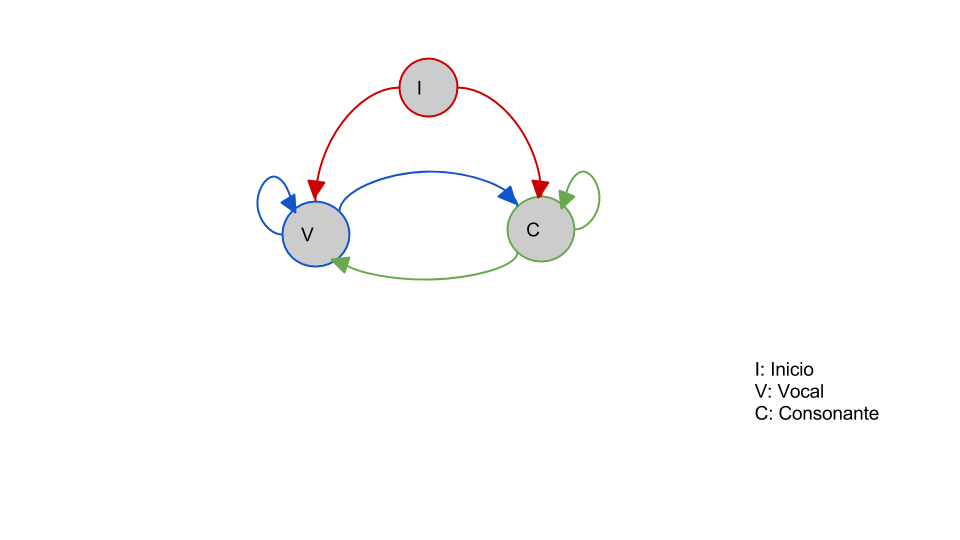
\includegraphics{../hmm/modelo_vocales.png}

\end{frame}

\begin{frame}{Paquetes utlizadas}

\begin{itemize}
\item
  Paquete HMM de R
\item
  Algoritmo de Baum-Welch para estimación de parámetros de una HMM
\end{itemize}

\end{frame}

\begin{frame}{Resultados Español}

Inicial sin conocimiento:

\begin{longtable}[c]{@{}ccc@{}}
\toprule\addlinespace
& V & C
\\\addlinespace
\midrule\endhead
& 0.5337 & 0.4662
\\\addlinespace
\bottomrule
\end{longtable}

Inicial después de Baum-Welch

\begin{longtable}[c]{@{}ccc@{}}
\toprule\addlinespace
& V & C
\\\addlinespace
\midrule\endhead
& 0.5337 & 0.4662
\\\addlinespace
\bottomrule
\end{longtable}

\end{frame}

\begin{frame}{Resultados Español}

Transiciones sin conocimiento

\begin{longtable}[c]{@{}ccc@{}}
\toprule\addlinespace
& V & C
\\\addlinespace
\midrule\endhead
V & 0.3099 & 0.6900
\\\addlinespace
C & 0.5200 & 0.4799
\\\addlinespace
\bottomrule
\end{longtable}

Transiciones después de Baum-Welch

\begin{longtable}[c]{@{}ccc@{}}
\toprule\addlinespace
& V & C
\\\addlinespace
\midrule\endhead
V & 0.3045 & 0.6954
\\\addlinespace
C & 0.993 & 0.006
\\\addlinespace
\bottomrule
\end{longtable}

\end{frame}

\begin{frame}{~Resultados Español}

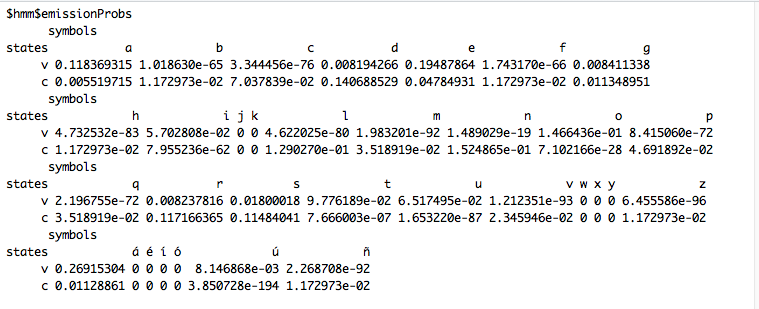
\includegraphics{../hmm/salida_vocales.png}

\end{frame}

\begin{frame}{~Resultado Griego}

Corpus:

\end{frame}

\begin{frame}{~Resultados Griego}

Inicial sin conocimiento:

\begin{longtable}[c]{@{}ccc@{}}
\toprule\addlinespace
& V & C
\\\addlinespace
\midrule\endhead
& 0.53765 & 0.4234
\\\addlinespace
\bottomrule
\end{longtable}

Inicial después de Baum-Welch

\begin{longtable}[c]{@{}ccc@{}}
\toprule\addlinespace
& V & C
\\\addlinespace
\midrule\endhead
& 0.6117 & 0.3882
\\\addlinespace
\bottomrule
\end{longtable}

\end{frame}

\begin{frame}{~Resultados Griego}

Transiciones sin conocimiento

\begin{longtable}[c]{@{}ccc@{}}
\toprule\addlinespace
& V & C
\\\addlinespace
\midrule\endhead
V & 0.3558 & 0.6441
\\\addlinespace
C & 0.5161 & 0.4838
\\\addlinespace
\bottomrule
\end{longtable}

Transiciones después de Baum-Welch

\begin{longtable}[c]{@{}ccc@{}}
\toprule\addlinespace
& V & C
\\\addlinespace
\midrule\endhead
V & 0.0093 & 0.9906
\\\addlinespace
C & 0.6178 & 0.3821
\\\addlinespace
\bottomrule
\end{longtable}

\end{frame}

\begin{frame}{Resultados Griego}

Vocales en griego

\begin{longtable}[c]{@{}cc@{}}
\toprule\addlinespace
Griego & Vocal
\\\addlinespace
\midrule\endhead
A,$\alpha$ & a
\\\addlinespace
E,$\epsilon$ & e
\\\addlinespace
I,$\iota$ & i
\\\addlinespace
O,$o$ & o
\\\addlinespace
Y,$\upsilon$ & u
\\\addlinespace
\bottomrule
\end{longtable}

\end{frame}

\begin{frame}{Resultados Griego}

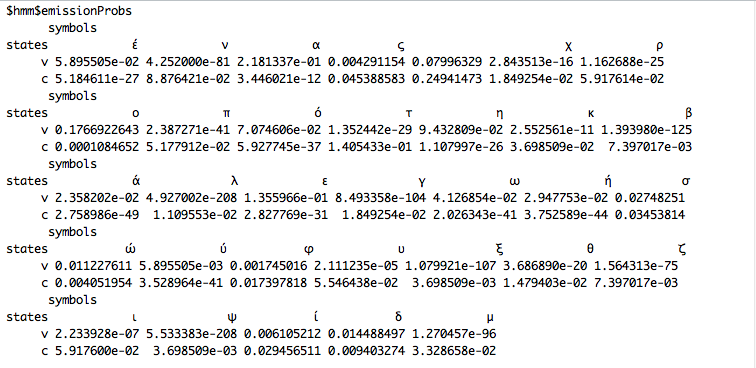
\includegraphics{../hmm/salida_vocales_griego.png}

\end{frame}

\section{Aplicación 2: Modelos jerárquicos y
postestratificación}\label{aplicacion-2-modelos-jerarquicos-y-postestratificacion}

\begin{frame}{Problema}

¿Cómo realizar inferencia sobre la población objetivo con datos de
encuesta recabados con un diseño no probabilístico basado en cuotas y
sin marco muestral?

\begin{block}{Objetivo}

\begin{itemize}
\itemsep1pt\parskip0pt\parsep0pt
\item
  Generar estimaciones precisas y confiables
\item
  Controlar por sesgo de selección
\end{itemize}

\end{block}

\end{frame}

\begin{frame}{Un poco de teoría de encuestas}

\begin{block}{Tipos de errores de encuestas}

\begin{itemize}
\itemsep1pt\parskip0pt\parsep0pt
\item
  Error de cobertura
\item
  Error de muestreo
\item
  Errores por no respuesta
\item
  Errores de medición
\end{itemize}

\end{block}

\begin{block}{Tipos de muestreo}

\begin{itemize}
\itemsep1pt\parskip0pt\parsep0pt
\item
  Probabilístico
\item
  No probabilístico
\end{itemize}

\end{block}

\end{frame}

\begin{frame}{No probabilístico por cuotas}

\textbf{Problema principal}: sesgo de selección.

$\Rightarrow$ Para hacer inferencias acerca de la población a partir de
una muestra de este tipo es necesario suponer que las personas que
fueron seleccionadas son similares a las que no lo fueron\ldots{}

\textbf{Soluciones posibles:}

\begin{itemize}
\itemsep1pt\parskip0pt\parsep0pt
\item
  Sample matching
\item
  Máximo entropía
\item
  MRP
\end{itemize}

\end{frame}

\begin{frame}{Especificación del modelo: pre MR}

Se denotará al estimador por este método como $\tilde{\theta}$ y se
obtiene con el siguiente proceso:

\begin{enumerate}
\def\labelenumi{\arabic{enumi}.}
\itemsep1pt\parskip0pt\parsep0pt
\item
  Identificación de una o más variables que pueden ser responsables del
  sesgo de selección. SPG, la cuadrícula completa de clasificación se
  trata como una única variable categórica $G$.
\end{enumerate}

\textbf{Limitación}: Con los datos de INEGI a nivel manzana solo podemos
especificar 5 modelos

\begin{itemize}
\itemsep1pt\parskip0pt\parsep0pt
\item
  Edad x colonia
\item
  Condición de ocupación x colonia
\item
  Escolaridad x colonia
\item
  Género x edad x colonia
\item
  Condición de ocupación x género x colonia
\end{itemize}

\end{frame}

\begin{frame}{¿Cómo se ven los datos?}

\textbf{Datos del censo}

\begin{itemize}
\itemsep1pt\parskip0pt\parsep0pt
\item
  Cuadricula: colonia x genero x edad
\item
  Dimensiones: 63 x 2 x 4 = 504
\end{itemize}

\begin{longtable}[c]{@{}lllr@{}}
\toprule\addlinespace
idcolonia & genero & edad & value
\\\addlinespace
\midrule\endhead
46241 & mujer & e12a17 & 38
\\\addlinespace
46284 & mujer & e12a17 & 0
\\\addlinespace
46385 & mujer & e12a17 & 171
\\\addlinespace
46388 & mujer & e12a17 & 124
\\\addlinespace
46408 & mujer & e12a17 & 74
\\\addlinespace
46409 & mujer & e12a17 & 108
\\\addlinespace
\bottomrule
\end{longtable}

\end{frame}

\begin{frame}{¿Cómo se ven los datos?}

\textbf{Datos de encuestas}

\begin{itemize}
\itemsep1pt\parskip0pt\parsep0pt
\item
  Datos individuales con las respuestas a los cuestionarios.
\item
  Las variables elegidas para $G$ se recodifican \emph{igualito} al
  censo.
\item
  La variable de interés en 0 y 1.
\item
  Morelos 2013: 5862
\item
  Morelos 2014: 10365
\end{itemize}

\begin{longtable}[c]{@{}lllr@{}}
\toprule\addlinespace
idcolonia & genero & edad & victimizacion
\\\addlinespace
\midrule\endhead
46548 & mujer & e18a29 & 0
\\\addlinespace
46548 & mujer & e12a17 & 1
\\\addlinespace
46548 & mujer & e30a49 & 1
\\\addlinespace
46284 & hombre & e30a49 & 0
\\\addlinespace
\bottomrule
\end{longtable}

\end{frame}

\begin{frame}{Especificación del modelo: el MR}

\begin{enumerate}
\def\labelenumi{\arabic{enumi}.}
\setcounter{enumi}{1}
\itemsep1pt\parskip0pt\parsep0pt
\item
  Se define un nuevo estimador
  $\gamma \equiv E(Y|D=d, G=g), d=1,...,J, g=1,...,G$.
\item
  Se utiliza un modelo de regresión multinivel apropiadamente
  especificado para estimar $\gamma$.
\end{enumerate}

\end{frame}

\begin{frame}{Especificación del modelo: el P}

\begin{enumerate}
\def\labelenumi{\arabic{enumi}.}
\setcounter{enumi}{3}
\itemsep1pt\parskip0pt\parsep0pt
\item
  El paso de postestratificación utiliza el modelo generado en el paso
  3. Se computa el estimador MRP para cada elemento $\theta_d$ de
  $\theta$ como la suma ponderada del subconjunto apropiado de
  $\hat{\gamma}$.
\end{enumerate}

\[
\tilde{\theta_d} = \sum_{g=1}^{G} \hat{\gamma_{d,g}} w_{g|d}
\]

donde $w_{g|d}=\frac{N_{g,d}}{N_d}$. El numerador es el número de
miembros de la población objetivo que pertenecen simultáneamente a la
categoría $g$ y $d$. El denominador es el número de miembros en la
población objetivo que pertenecen a la categoría $d$.

\end{frame}

\begin{frame}{Resultados}

Muestras no comparables, ¡ahora lo son!

\begin{longtable}[c]{@{}lrrrr@{}}
\toprule\addlinespace
& e12a17 & e18a29 & e30a49 & e50omas
\\\addlinespace
\midrule\endhead
Hombres.14 & 17.8684843 & 21.9930360 & 23.452651 & 20.998060
\\\addlinespace
Hombres.13 & 18.4638051 & 21.4389763 & 27.861405 & 22.353171
\\\addlinespace
Diferencia & -0.5953207 & 0.5540598 & -4.408754 & -1.355112
\\\addlinespace
Mujeres.14 & 14.9715021 & 18.4999490 & 19.796484 & 17.682535
\\\addlinespace
Mujeres.13 & 17.1969776 & 19.9538614 & 26.118268 & 20.920638
\\\addlinespace
Diferencia & -2.2254755 & -1.4539125 & -6.321784 & -3.238104
\\\addlinespace
\bottomrule
\end{longtable}

\end{frame}

\begin{frame}{MRP}

\textbf{Resuelve:} small area estimation y/o selection bias

\textbf{Ventajas del método}

\begin{itemize}
\itemsep1pt\parskip0pt\parsep0pt
\item
  El uso de la regresión multinivel incrementa la precisión del
  estimador.
\item
  Si $G$ se define adecuadamente, la postestratificación ayuda a
  decrecer el error por sesgo de selección.
\item
  MRP es un estimador relativamente preciso para $\theta$.
\end{itemize}

\textbf{Desventajas del método}

\begin{itemize}
\itemsep1pt\parskip0pt\parsep0pt
\item
  Se necesitan datos poblacionales para toda la clasificación $DxG$ lo
  cuál limita la definición de $G$.
\item
  Para obtener buenos estimadores de $\gamma$, el modelo de regresión
  multinivel debe ser especificado con mucho cuidado. Sin embargo, esta
  limitación aplica para cualquier modelo.
\end{itemize}

\end{frame}

\end{document}
